\documentclass{anstrans}
%%%%%%%%%%%%%%%%%%%%%%%%%%%%%%%%%%%
\title{Online reprocessing simulation for thorium-fueled molten salt breeder reactor}

\author{Andrei Rykhlevskii, Alexander Lindsay, Kathryn Huff}

\institute{
Department of Nuclear, Plasma, and Radiological Engineering, University of Illinois at Urbana-Champaign \break
Urbana, IL
}

\email{andreir2@illinois.edu}

%%%% packages and definitions (optional)
\usepackage{graphicx} % allows inclusion of graphics
\usepackage{caption}  % allows center figures caption
\usepackage{booktabs} % nice rules (thick lines) for tables
\usepackage{microtype} % improves typography for PDF
\usepackage[section]{placeins}

\usepackage[acronym,toc]{glossaries}  % acronyms inclusion
%\newacronym{<++>}{<++>}{<++>}
\newacronym[longplural={metric tons of heavy metal}]{MTHM}{MTHM}{metric ton of heavy metal}
\newacronym{ABM}{ABM}{agent-based modeling}
\newacronym{ACDIS}{ACDIS}{Program in Arms Control \& Domestic and International Security}
\newacronym{AHTR}{AHTR}{Advanced High Temperature Reactor}
\newacronym{ANDRA}{ANDRA}{Agence Nationale pour la gestion des D\'echets RAdioactifs, the French National Agency for Radioactive Waste Management}
\newacronym{ANL}{ANL}{Argonne National Laboratory}
\newacronym{ANS}{ANS}{American Nuclear Society}
\newacronym{API}{API}{application programming interface}
\newacronym{ARE}{ARE}{Aircraft Reactor Experiment}
\newacronym{ARFC}{ARFC}{Advanced Reactors and Fuel Cycles}
\newacronym{ASME}{ASME}{American Society of Mechanical Engineers}
\newacronym{ATWS}{ATWS}{Anticipated Transient Without Scram}
\newacronym{BDBE}{BDBE}{Beyond Design Basis Event}
\newacronym{BIDS}{BIDS}{Berkeley Institute for Data Science}
\newacronym{CAFCA}{CAFCA}{ Code for Advanced Fuel Cycles Assessment }
\newacronym{CDTN}{CDTN}{Centro de Desenvolvimento da Tecnologia Nuclear}
\newacronym{CEA}{CEA}{Commissariat \`a l'\'Energie Atomique et aux \'Energies Alternatives}
\newacronym{CI}{CI}{continuous integration}
\newacronym{CNEN}{CNEN}{Comiss\~{a}o Nacional de Energia Nuclear}
\newacronym{CNERG}{CNERG}{Computational Nuclear Engineering Research Group}
\newacronym{COSI}{COSI}{Commelini-Sicard}
\newacronym{COTS}{COTS}{commercial, off-the-shelf}
\newacronym{CSNF}{CSNF}{commercial spent nuclear fuel}
\newacronym{CTAH}{CTAHs}{Coiled Tube Air Heaters}
\newacronym{CUBIT}{CUBIT}{CUBIT Geometry and Mesh Generation Toolkit}
\newacronym{CURIE}{CURIE}{Centralized Used Fuel Resource for Information Exchange}
\newacronym{DAG}{DAG}{directed acyclic graph}
\newacronym{DANESS}{DANESS}{Dynamic Analysis of Nuclear Energy System Strategies}
\newacronym{DBE}{DBE}{Design Basis Event}
\newacronym{DESAE}{DESAE}{Dynamic Analysis of Nuclear Energy Systems Strategies}
\newacronym{DHS}{DHS}{Department of Homeland Security}
\newacronym{DOE}{DOE}{Department of Energy}
\newacronym{DRACS}{DRACS}{Direct Reactor Auxiliary Cooling System}
\newacronym{DRE}{DRE}{dynamic resource exchange}
\newacronym{DSNF}{DSNF}{DOE spent nuclear fuel}
\newacronym{DYMOND}{DYMOND}{Dynamic Model of Nuclear Development }
\newacronym{EBS}{EBS}{Engineered Barrier System}
\newacronym{EDF}{EDF}{Électricité de France}
\newacronym{EDZ}{EDZ}{Excavation Disturbed Zone}
\newacronym{EIA}{EIA}{U.S. Energy Information Administration}
\newacronym{EPA}{EPA}{Environmental Protection Agency}
\newacronym{EPR}{EPR}{European Pressurized Reactors}
\newacronym{EP}{EP}{Engineering Physics}
\newacronym{EU}{EU}{European Union}
\newacronym{FCO}{FCO}{Fuel Cycle Options}
\newacronym{FCT}{FCT}{Fuel Cycle Technology}
\newacronym{FEHM}{FEHM}{Finite Element Heat and Mass Transfer}
\newacronym{FEPs}{FEPs}{Features, Events, and Processes}
\newacronym{FHR}{FHR}{Fluoride-Salt-Cooled High-Temperature Reactor}
\newacronym{FLiBe}{FLiBe}{Fluoride-Lithium-Beryllium}
\newacronym{FP}{FP}{Fission Products}
\newacronym{GDSE}{GDSE}{Generic Disposal System Environment}
\newacronym{GDSM}{GDSM}{Generic Disposal System Model}
\newacronym{GENIUSv1}{GENIUSv1}{Global Evaluation of Nuclear Infrastructure Utilization Scenarios, Version 1}
\newacronym{GENIUSv2}{GENIUSv2}{Global Evaluation of Nuclear Infrastructure Utilization Scenarios, Version 2}
\newacronym{GENIUS}{GENIUS}{Global Evaluation of Nuclear Infrastructure Utilization Scenarios}
\newacronym{GPAM}{GPAM}{Generic Performance Assessment Model}
\newacronym{GRSAC}{GRSAC}{Graphite Reactor Severe Accident Code}
\newacronym{GUI}{GUI}{graphical user interface}
\newacronym{HLW}{HLW}{high level waste}
\newacronym{HPC}{HPC}{high-performance computing}
\newacronym{HTC}{HTC}{high-throughput computing}
\newacronym{HTGR}{HTGR}{High Temperature Gas-Cooled Reactor}
\newacronym{IAEA}{IAEA}{International Atomic Energy Agency}
\newacronym{IEMA}{IEMA}{Illinois Emergency Mangament Agency}
\newacronym{IHLRWM}{IHLRWM}{International High Level Radioactive Waste Management}
\newacronym{INL}{INL}{Idaho National Laboratory}
\newacronym{IPRR1}{IRP-R1}{Instituto de Pesquisas Radioativas Reator 1}
\newacronym{IRP}{IRP}{Integrated Research Project}
\newacronym{ISFSI}{ISFSI}{Independent Spent Fuel Storage Installation}
\newacronym{ISRG}{ISRG}{Independent Student Research Group}
\newacronym{JFNK}{JFNK}{Jacobian-Free Newton Krylov}
\newacronym{LANL}{LANL}{Los Alamos National Laboratory}
\newacronym{LBNL}{LBNL}{Lawrence Berkeley National Laboratory}
\newacronym{LCOE}{LCOE}{levelized cost of electricity}
\newacronym{LDRD}{LDRD}{laboratory directed research and development}
\newacronym{LFR}{LFR}{Lead-Cooled Fast Reactor}
\newacronym{LLNL}{LLNL}{Lawrence Livermore National Laboratory}
\newacronym{LMFBR}{LMFBR}{Liquid Metal Fast Breeder Reactor}
\newacronym{LOFC}{LOFC}{Loss of Forced Cooling}
\newacronym{LOHS}{LOHS}{Loss of Heat Sink}
\newacronym{LOLA}{LOLA}{Loss of Large Area}
\newacronym{LP}{LP}{linear program}
\newacronym{LWR}{LWR}{Light Water Reactor}
\newacronym{MAGNOX}{MAGNOX}{Magnesium Alloy Graphie Moderated Gas Cooled Uranium Oxide Reactor}
\newacronym{MA}{MA}{minor actinide}
\newacronym{MCNP}{MCNP}{Monte Carlo N-Particle code}
\newacronym{MILP}{MILP}{mixed-integer linear program}
\newacronym{MIT}{MIT}{the Massachusetts Institute of Technology}
\newacronym{MOAB}{MOAB}{Mesh-Oriented datABase}
\newacronym{MOOSE}{MOOSE}{Multiphysics Object-Oriented Simulation Environment}
\newacronym{MOX}{MOX}{mixed oxide}
\newacronym{MSBR}{MSBR}{Molten Salt Breeder Reactor}
\newacronym{MSRE}{MSRE}{Molten Salt Reactor Experiment}
\newacronym{MSR}{MSR}{Molten Salt Reactor}
\newacronym{NAGRA}{NAGRA}{National Cooperative for the Disposal of Radioactive Waste}
\newacronym{NEAMS}{NEAMS}{Nuclear Engineering Advanced Modeling and Simulation}
\newacronym{NEUP}{NEUP}{Nuclear Energy University Programs}
\newacronym{NFCSim}{NFCSim}{Nuclear Fuel Cycle Simulator}
\newacronym{NGNP}{NGNP}{Next Generation Nuclear Plant}
\newacronym{NMWPC}{NMWPC}{Nuclear MW Per Capita}
\newacronym{NNSA}{NNSA}{National Nuclear Security Administration}
\newacronym{NPP}{NPP}{Nuclear Power Plant}
\newacronym{NPRE}{NPRE}{Department of Nuclear, Plasma, and Radiological Engineering}
\newacronym{NQA1}{NQA-1}{Nuclear Quality Assurance - 1}
\newacronym{NRC}{NRC}{Nuclear Regulatory Commission}
\newacronym{NSF}{NSF}{National Science Foundation}
\newacronym{NSSC}{NSSC}{Nuclear Science and Security Consortium}
\newacronym{NUWASTE}{NUWASTE}{Nuclear Waste Assessment System for Technical Evaluation}
\newacronym{NWF}{NWF}{Nuclear Waste Fund}
\newacronym{NWTRB}{NWTRB}{Nuclear Waste Technical Review Board}
\newacronym{OCRWM}{OCRWM}{Office of Civilian Radioactive Waste Management}
\newacronym{ORION}{ORION}{ORION}
\newacronym{ORNL}{ORNL}{Oak Ridge National Laboratory}
\newacronym{PARCS}{PARCS}{Purdue Advanced Reactor Core Simulator}
\newacronym{PBAHTR}{PB-AHTR}{Pebble Bed Advanced High Temperature Reactor}
\newacronym{PBFHR}{PB-FHR}{Pebble-Bed Fluoride-Salt-Cooled High-Temperature Reactor}
\newacronym{PEI}{PEI}{Peak Environmental Impact}
\newacronym{PH}{PRONGHORN}{PRONGHORN}
\newacronym{PRIS}{PRIS}{Power Reactor Information System}
\newacronym{PRKE}{PRKE}{Point Reactor Kinetics Equations}
\newacronym{PSPG}{PSPG}{Pressure-Stabilizing/Petrov-Galerkin}
\newacronym{PWAR}{PWAR}{Pratt and Whitney Aircraft Reactor}
\newacronym{PWR}{PWR}{Pressurized Water Reactor}
\newacronym{PyNE}{PyNE}{Python toolkit for Nuclear Engineering}
\newacronym{PyRK}{PyRK}{Python for Reactor Kinetics}
\newacronym{QA}{QA}{quality assurance}
\newacronym{RDD}{RD\&D}{Research Development and Demonstration}
\newacronym{RD}{R\&D}{Research and Development}
\newacronym{RELAP}{RELAP}{Reactor Excursion and Leak Analysis Program}
\newacronym{RIA}{RIA}{Reactivity Insertion Accident}
\newacronym{RIF}{RIF}{Region-Institution-Facility}
\newacronym{SFR}{SFR}{Sodium-Cooled Fast Reactor}
\newacronym{SINDAG}{SINDA{\textbackslash}G}{Systems Improved Numerical Differencing Analyzer $\backslash$ Gaski}
\newacronym{SKB}{SKB}{Svensk K\"{a}rnbr\"{a}nslehantering AB}
\newacronym{SNF}{SNF}{spent nuclear fuel}
\newacronym{SNL}{SNL}{Sandia National Laboratory}
\newacronym{STC}{STC}{specific temperature change}
\newacronym{SUPG}{SUPG}{Streamline-Upwind/Petrov-Galerkin}
\newacronym{SWF}{SWF}{Separations and Waste Forms}
\newacronym{SWU}{SWU}{Separative Work Unit}
\newacronym{TRIGA}{TRIGA}{Training Research Isotope General Atomic}
\newacronym{TRISO}{TRISO}{Tristructural Isotropic}
\newacronym{TSM}{TSM}{Total System Model}
\newacronym{TSPA}{TSPA}{Total System Performance Assessment for the Yucca Mountain License Application}
\newacronym{ThOX}{ThOX}{thorium oxide}
\newacronym{UFD}{UFD}{Used Fuel Disposition}
\newacronym{UML}{UML}{Unified Modeling Language}
\newacronym{UOX}{UOX}{uranium oxide}
\newacronym{UQ}{UQ}{uncertainty quantification}
\newacronym{US}{US}{United States}
\newacronym{UW}{UW}{University of Wisconsin}
\newacronym{VISION}{VISION}{the Verifiable Fuel Cycle Simulation Model}
\newacronym{VVER}{VVER}{Voda-Vodyanoi Energetichesky Reaktor (Russian Pressurized Water Reactor)}
\newacronym{VV}{V\&V}{verification and validation}
\newacronym{WIPP}{WIPP}{Waste Isolation Pilot Plant}
\newacronym{YMR}{YMR}{Yucca Mountain Repository Site}

	
\makeglossaries

\graphicspath{{figures/}}

\newcommand{\SN}{S$_N$}
\renewcommand{\vec}[1]{\bm{#1}} %vector is bold italic
\newcommand{\vd}{\bm{\cdot}} % slightly bold vector dot
\newcommand{\grad}{\vec{\nabla}} % gradient
\newcommand{\ud}{\mathop{}\!\mathrm{d}} % upright derivative symbol

\begin{document}
%%%%%%%%%%%%%%%%%%%%%%%%%%%%%%%%%%%%%%%%%%%%%%%%%%%%%%%%%%%%%%%%%%%%%%%%%%%%%%%%
\section{Introduction}
The thermal spectrum \gls{MSR} is an advanced type of reactor consist of constantly circulating liquid fuel (i.e., mixture of $LiF-BeF_2-ThF_4-UF_4$ or $LiF-BeF_2-ZrF_4-UF_4$) which works also as a coolant, and the reactor graphite as moderator. This fuel form leads to immediate advantages over traditional, solid-fueled, reactors. The molten-salt carrier salt with dissolved in it fissile and/or fertile material allows to use online refuelling and reprocessing, which means \gls{MSR}s can operate years without shutdown, achieve maximum fuel utilization, and outstanding neutron economy \cite{leblanc_molten_2010}. Moreover, this type of fuel does not need fabrication and could be transported from enrichment plant to \gls{NPP} in form of uranium hexafluoride ($UF_6$), so \gls{MSR}s are also beneficial with regards to economics. Additionally, it has high level of inherent safety due to strong negative temeperature coefficient of reactivity, near-atmospheric pressure in the primary loop, stable coolant, passive decay heat cooling, and small excess reactivity \cite{elsheikh_safety_2013}.

The thorium fueled Molten Salt Breeder Reactor (MSBR) was developed in early 1970s specifically to realize the promise of the thorium fuel cycle which allows the use of natural thorium instead of enriched uranium as the fertile element. Thorium breeds the fissile $^{233}U$ and avoids uranium enrichment \cite{robertson_conceptual_1971}. In the matter of nuclear fuel cycle, the thorium cycle produces much less amount of plutonium and minor actinides (MAs) comparing to the traditional uranium fuel cycle, consequently, it might significantly increase prolifiration resistance when \gls{MSR} operates in the breeder regime. The \gls{MSR}s also could be employed as converter reactor for transmutation spent fuel from \gls{LWR} or others.

Nowadays, interest to \gls{MSR} coming back after long-term break because of its unique characteristics and features of this type of reactor, such as online reprocessing and refueling. For the development of \gls{MSR} conception special computational analysis methods and codes needed due to completely different physics of liquid-fueled nuclear reactor comparing with traditional, solid-fueled, reactors. Most of the contemporary nuclear reactor physics codes do not able to perform depletion calculations in the online reprocessing regime. J.J. Powers (\gls{ORNL}) has suggested a novel method to conducting depletion simulation for \gls{MSR} with taking into account the online reprocessing and refueling based on the deterministic computer code NEWT in SCALE \cite{powers_new_2013}. This approach was later used by Jeong et al. to find equilibrium state for MSBR and validate it with MCNP6/CINDER90 model \cite{jeong_equilibrium_2016}. For the development of MSBR research, this paper presents the MSBR single-cell model developed using a continuous-energy the Serpent 2 Monte Carlo reactor physics calculation code that was employed to find equilibrium core state, and several calculation results including the depletion calculation of the single-cell unit.

All calculations presented in this paper were performed using the Serpent 2 code version 2.1.29 with ENDF/B-VII
nuclear data \cite{leppanen_serpent_2012,chadwick_endf/b-vii.0:_2006}. Compared with Serpent 1, Serpent 2 has many more useful features and contains a complete redesign of memory management using hybrid OpenMP + MPI parallelization, which is important in depletion calculations using computer clusters with multiple cores \cite{leppanen_serpent_2015}. This paper use build-in Serpent 2 depletion capabilities with online reprocessing subroutine. Another feature, circulating
liquid fuel, which causes delayed neutron precursor drift is not treated here.

%%%%%%%%%%%%%%%%%%%%%%%%%%%%%%%%%%%%%%%%%%%%%%%%%%%%%%%%%%%%%%%%%%%%%%%%%%%%%%%%
\section{MSBR design description}
The MSBR vessel has diameter of 680 cm and a height of 610 cm. It contains molten fluoride fuel-salt mixture which performs two functions: to generate heat in the moderated region and to transport heat energy from the core to primary heat exchanger using the primary salt pump. The vessel also contains graphite blocks for neutron moderation and reflection. The reactor core has a central zone, Zone I, in which 13\% of the volume is fuel salt and 87\% graphite. The first zone is composed of 1320 graphite cells, 2 graphite control rods, and 2 safety rods consisting of boron carbide clad. The undermoderated zone, Zone II, with 37\% fuel salt, and radial reflector, surrounding the more active portion serves to diminish neutron leakage from the reactor core. This zone is formed of two kinds of elements: elements like those in Zone I except for a larger hole size (Zone II-A), and radially spread graphite slats (Zone II-B). At the outer of the core there are graphite reflector and vessel wall. Between the core and the reflector blocks located annulus which is 100\% salt needed to provide possibility removing and inserting a graphite assembly. 

Figure~\ref{fig:plan} shows the plan view of the whole-core configuration at the expected reactor operational level when all control rods are fully withdrawn from the core.  Figure~\ref{fig:elevation} shows the longitudinal section of the reactor. The violet color represents bare graphite, and the yellow represents fuel salt. The blue color shows Hastelloy-N, a material used for the plenum and vessel wall, and the black color is a void space. All figures of the core in this work generated using built-in Serpent plotter.
\begin{figure}[!htb] % replace 't' with 'b' to force it to be on the bottom
  \centering
  \vspace{-0.6em}
  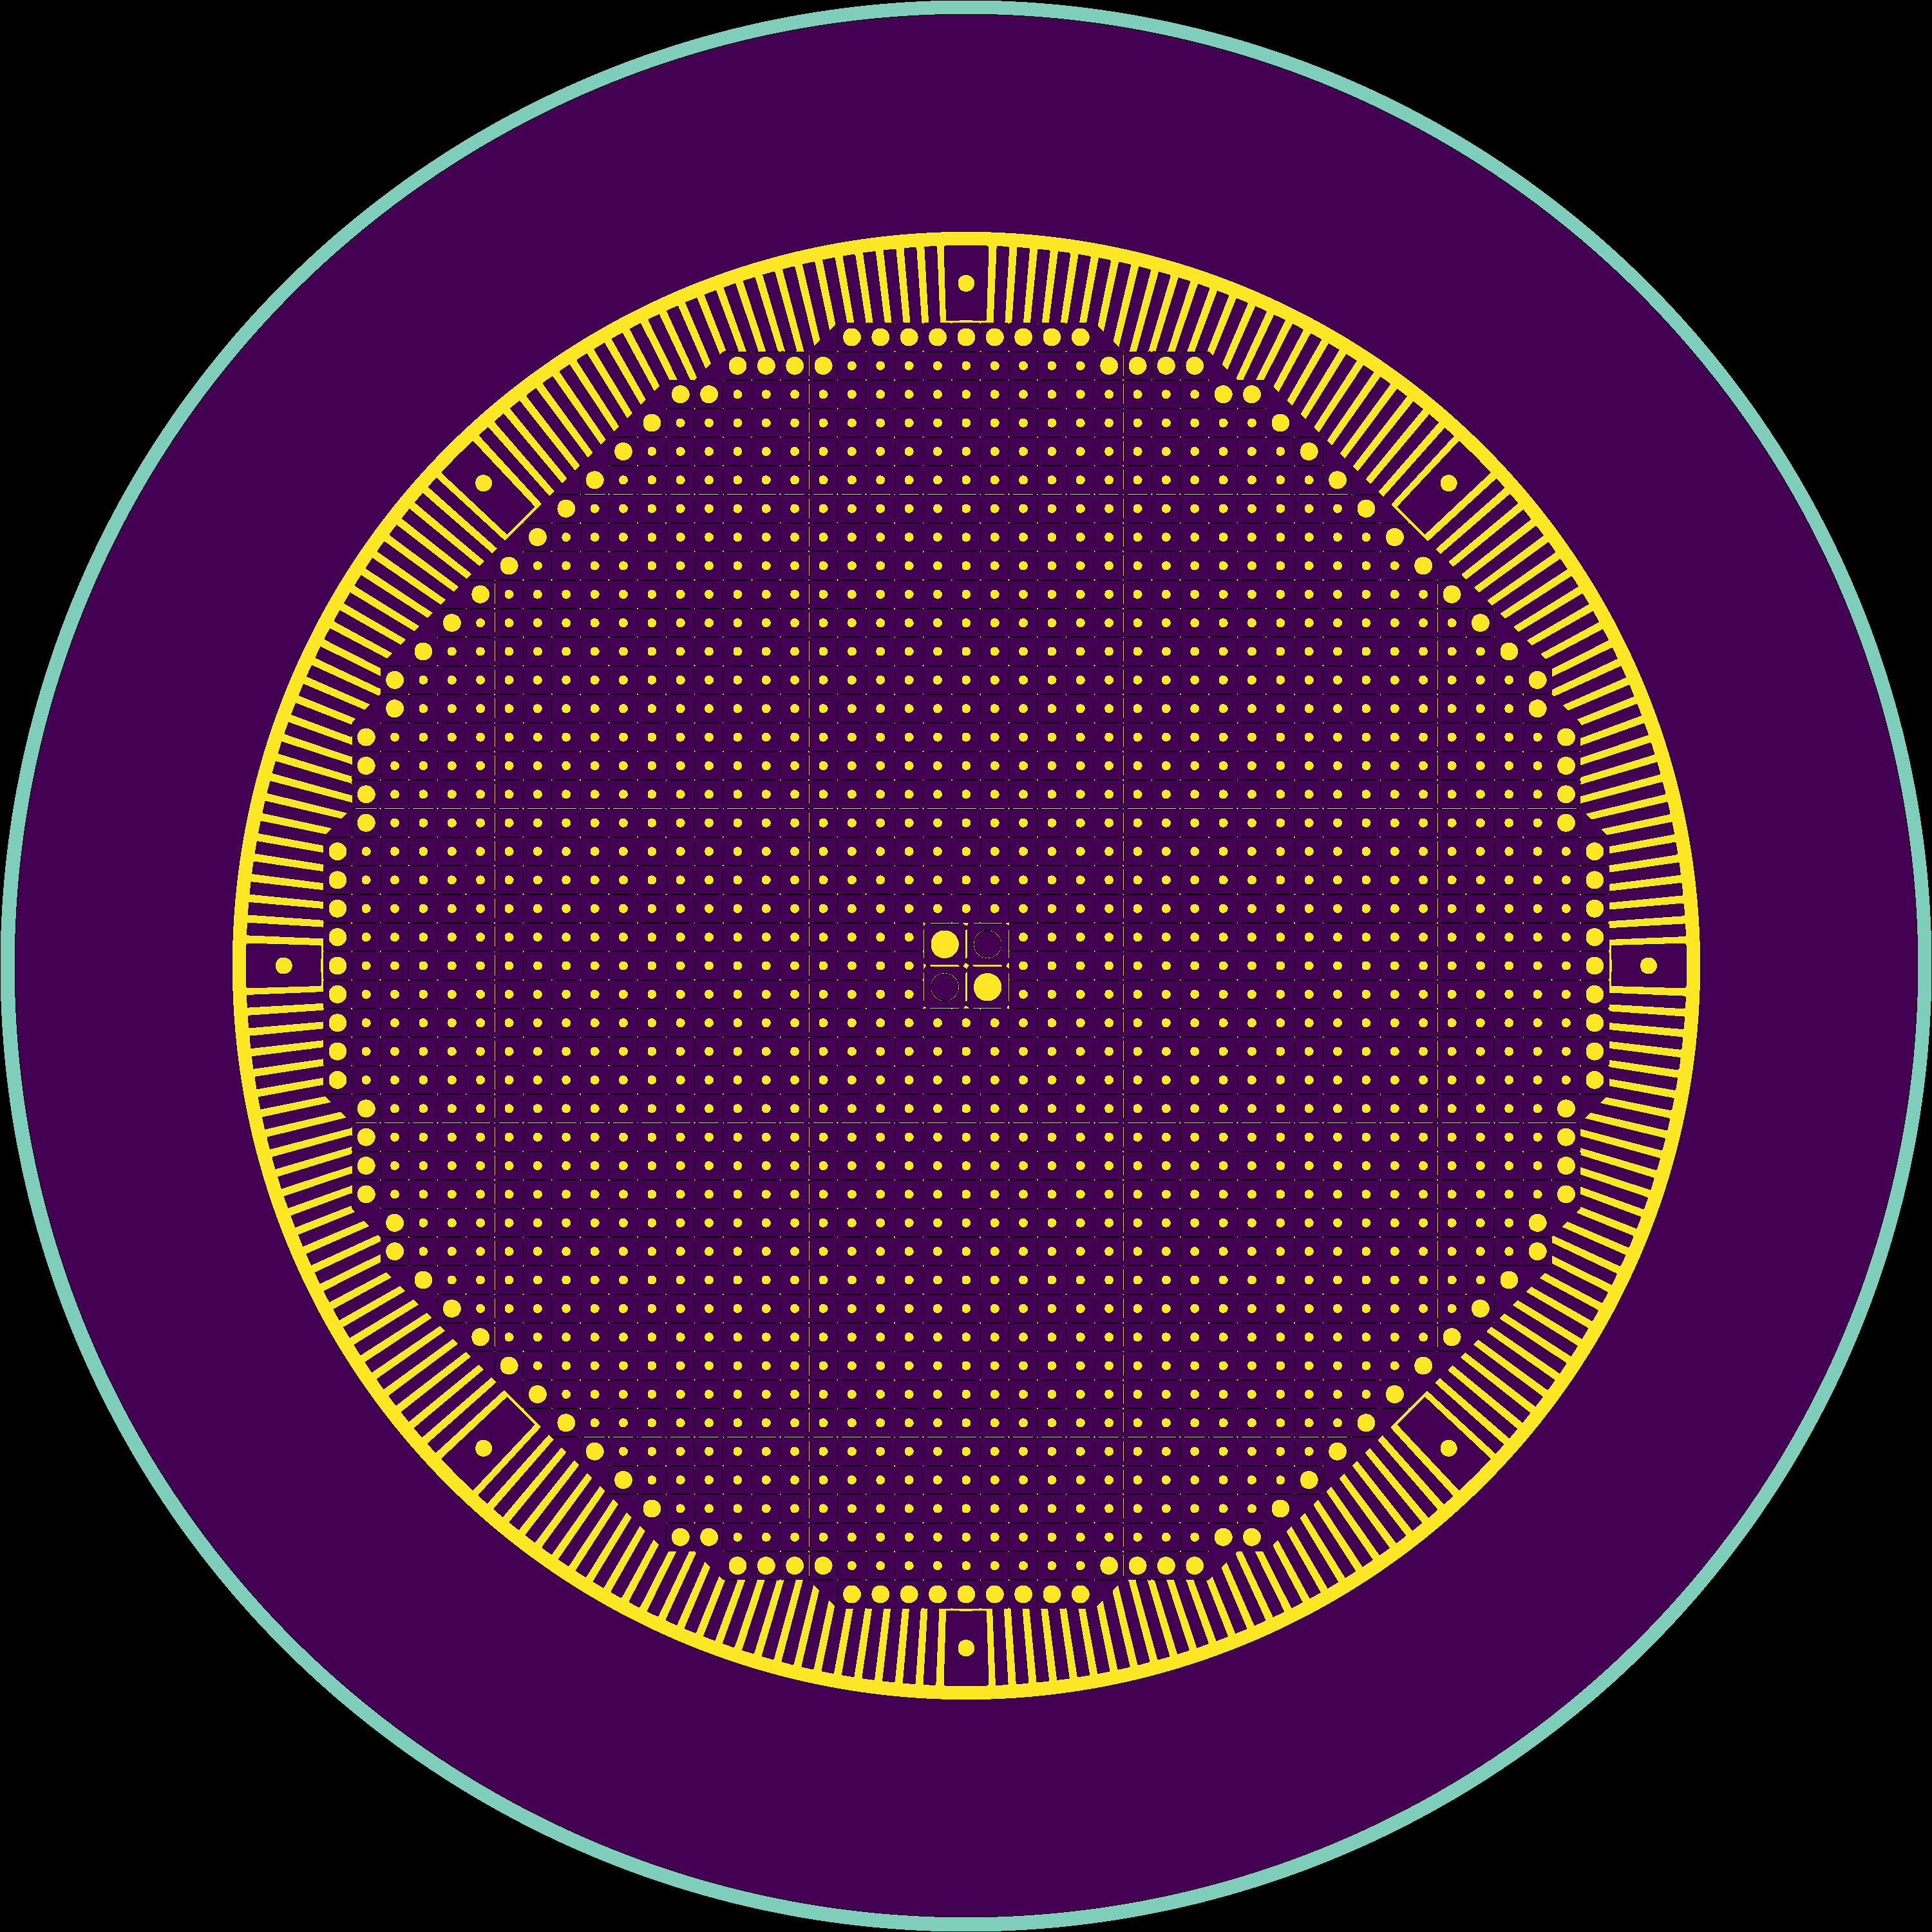
\includegraphics[width=0.93\linewidth]{figure_2_1.png}
  \caption{Plan view of MSBR core.}
  \label{fig:plan}
\end{figure}

\begin{figure}[ht] % replace 't' with 'b' to force it to be on the bottom
  \centering
  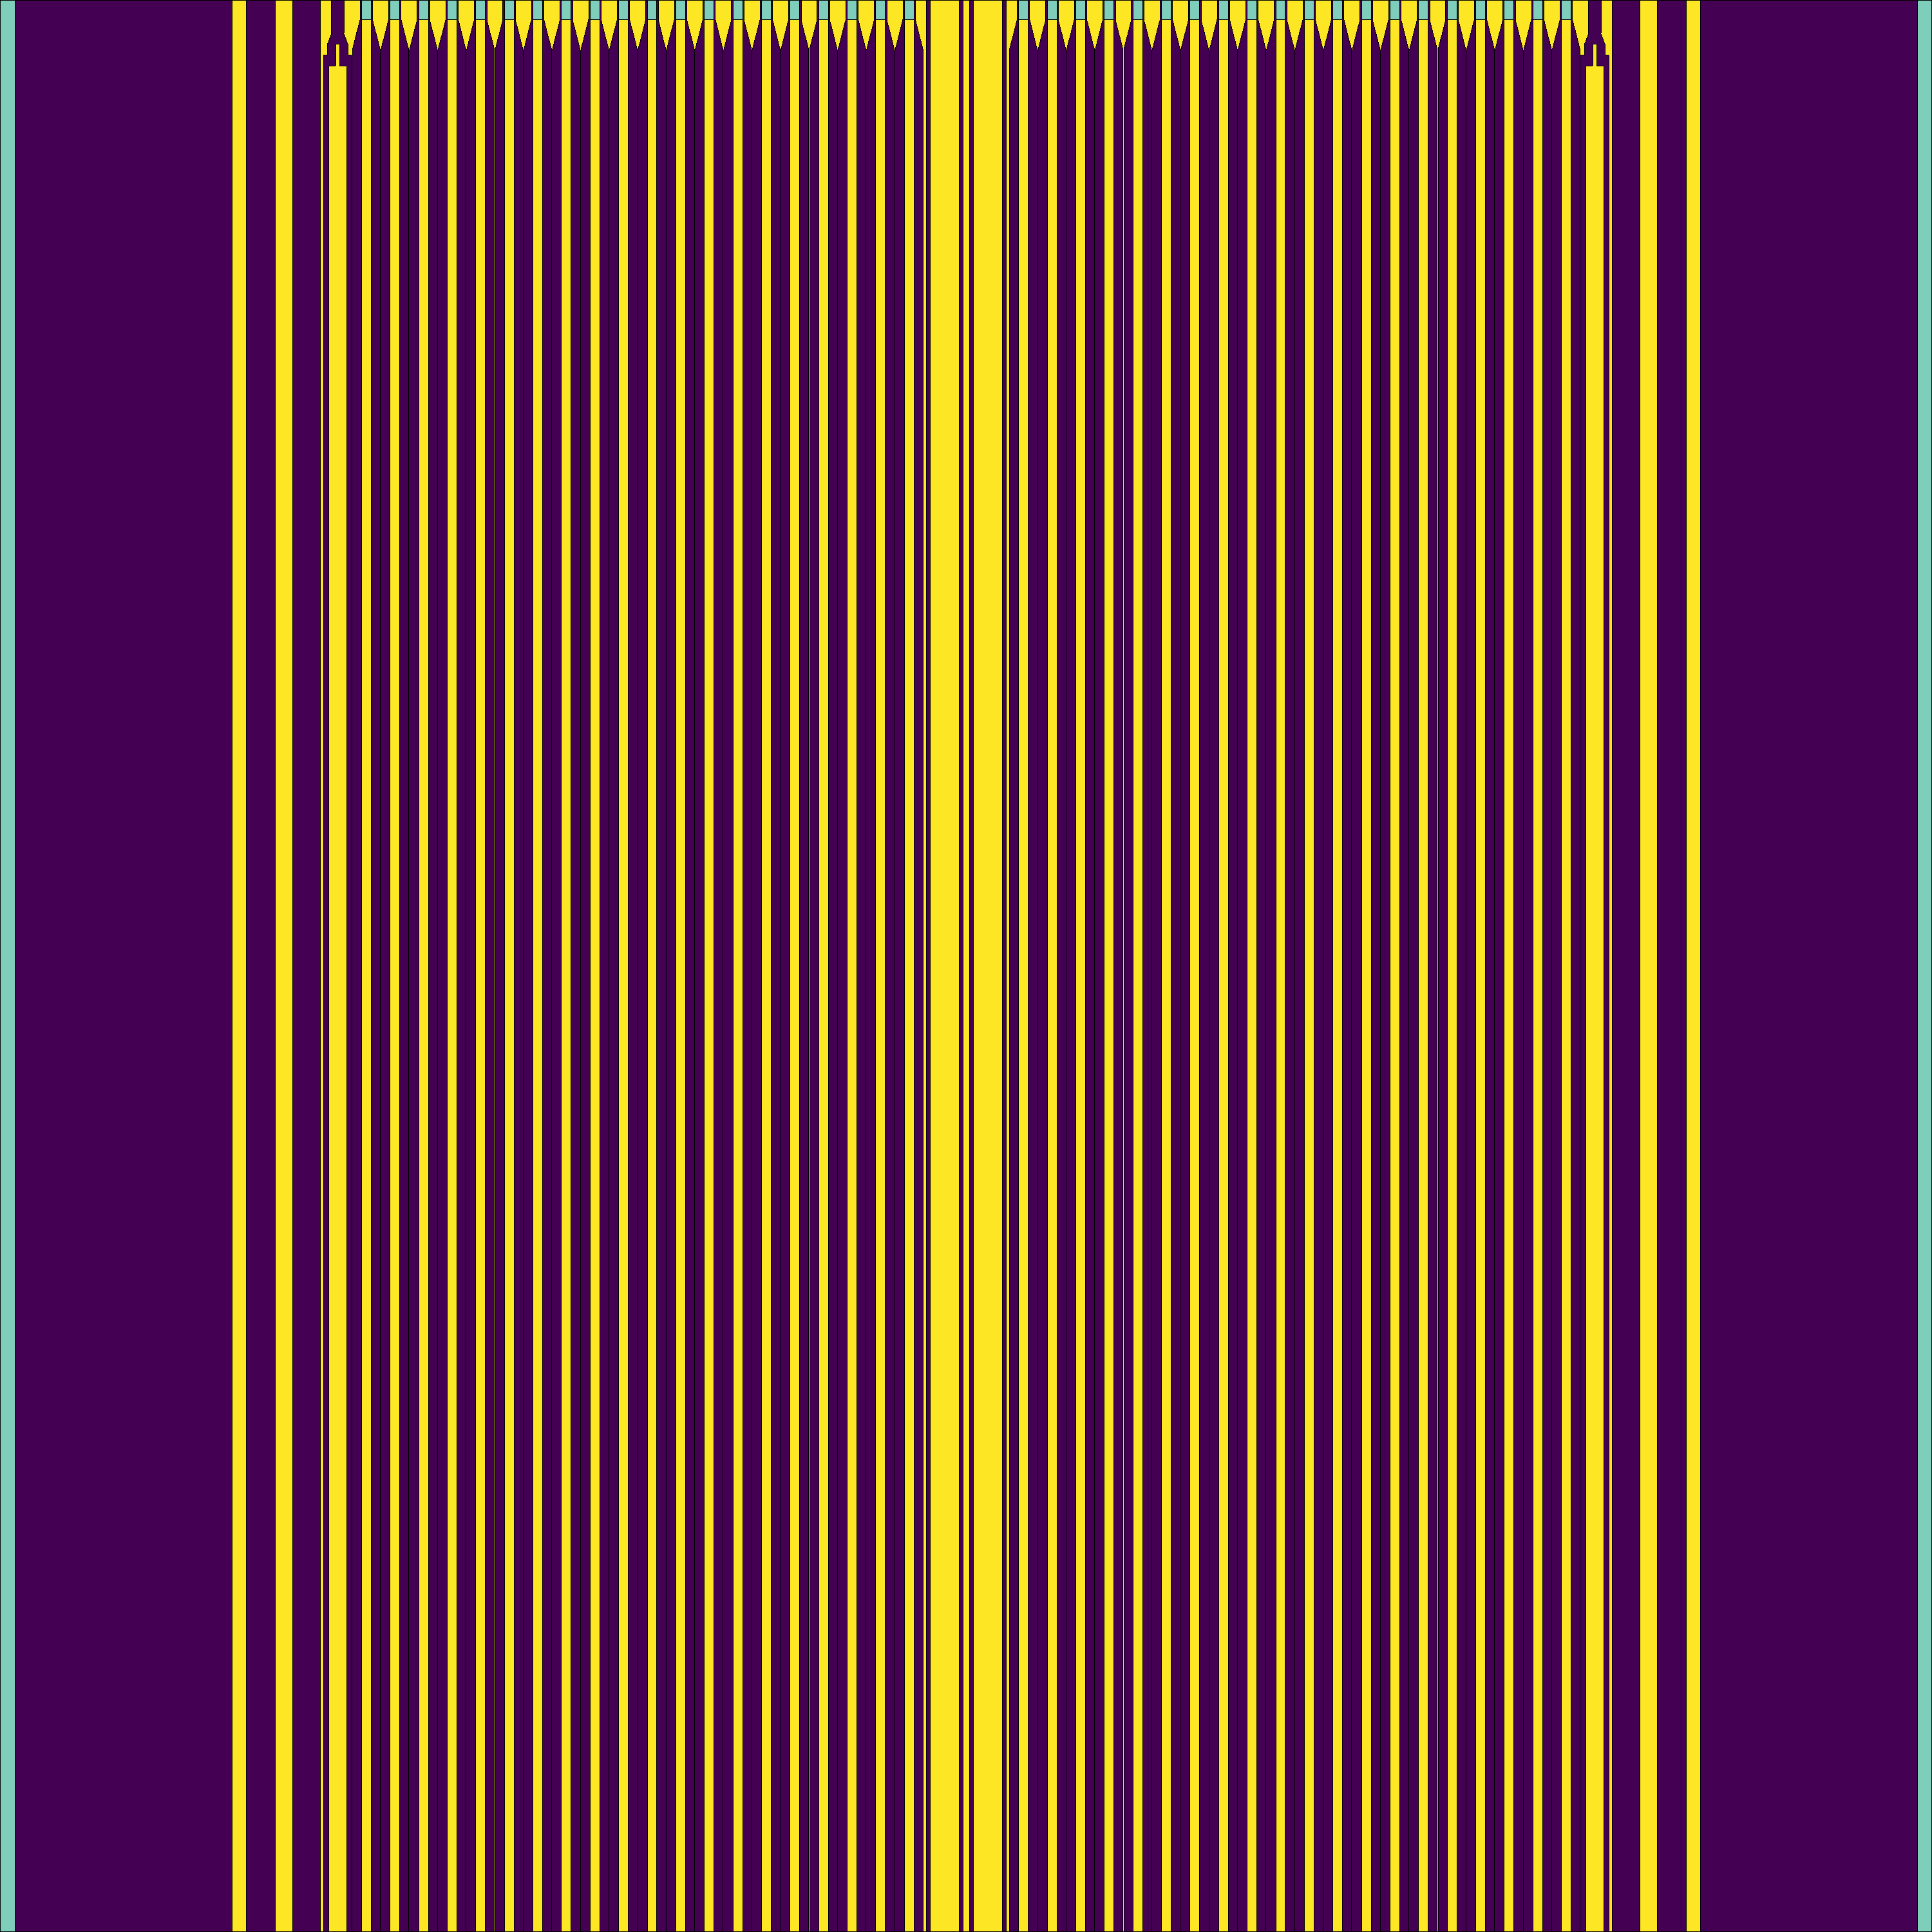
\includegraphics[width=\linewidth]{figure_2_2.png}
  \caption{Elevation view of MSBR core.}
  \label{fig:elevation}
\end{figure}

\subsection{Core Zone I and II-A}
The central portion, called Zone I, is made up of $10.16cm\times10.16cm\times396.24cm$-long graphite elements. The fuel salt to graphite volume ratio of Zone I is 13.2\%, and the central hole has a diameter of $3.42cm$. Zone II has 37\% salt and central hole diameter of $6.604cm$. Both types of elements mostly have a rectangular shape with a part of cylinder sticking out at each corner to form salt flow between the graphite channels. Different sizes of elements are necessary to reduce the peak damage flux and power density in the center of the core to prevent local graphite damage. Figure~\ref{fig:zone12A} demonstrates the reconstructed graphite element utilized for this Monte Carlo model.

\begin{figure}[h] % replace 't' with 'b' to force it to be on the bottom
  \centering
  
\includegraphics[width=0.96\linewidth]{figure_2_4.png}
  \caption{Zone I (left) and Zone II-A (right) elements.}
  \label{fig:zone12A}
\end{figure}

\subsection{Core Zone II-B}
The second core zone is divided into two different zones: Zone II-A and Zone II-B. The graphite elements for Zone II-A are prismatic and form the first reflecting layer surrounding the core zone I. The elements for zone II-B made up in the form of rectangular slats spaced far enough apart to achieve 0.37 fuel salt volume fraction. Figure~\ref{fig:zone2B} shows the outer Zone II, 5.08cm-wide annular space between the core graphite and the radial reflector graphite. The annulus contains 100\% fuel salt and serves to reduce the damage flux at the internal surface of the graphite reflector blocks. The reactor Zone II-B graphite $5.08cm$-thick slats and various length in width (average width is about $26.67cm$) are reconstructed as is in the model without any approximation. From the ORNL report \cite{robertson_conceptual_1971}, the suggested design of Zone II-B has 8 graphite elements every $45^\circ$ with irregular shape as well as holes for the flow of salt and were simplified into a right circular hollow cylinder sector shape with the central hole. This is only simplification for this model.

\subsection{Material composition}
The fuel salt, the reactor graphite, and the modified Hastelloy N are exclusive MSBR materials which were created at ORNL. The isotope composition of each material at the initial state was described in detail in the MSBR conceptual design study \cite{robertson_conceptual_1971} and has been applied to Serpent model without any modification. 

\begin{figure}[hb] % replace 't' with 'b' to force it to be on the bottom
  \centering
  
\includegraphics[width=0.93\linewidth]{figure_2_5.png}
  \caption{Plan view of Zone II-B.}
  \label{fig:zone2B}
\end{figure}

The initial fuel salt loading composition is $LiF-BeF_2-ThF_4-^{233}UF_4-^{239}PuF_3$ (72-16-12-0.232-0.0006 mole \%). The lithium is enriched to 99.995\% $^{7}Li$ because $^{6}Li$ is a very strong neutron poison and becomes tritium upon neutron bombardment. In this study, the 0.005\% atomic fraction of $^{6}Li$ has been taken into account because even such a small amount of isotope with very high absorption cross section might significantly affect on effective multiplication factor. For cross section data generation ENDF/B-VII was employed \cite{chadwick_endf/b-vii.0:_2006}. %Specific temperature was fixed for each material to correctly model the Doppler-broadening of resonance peaks when Serpent generate problem-oriented nuclear data library.

%%%%%%%%%%%%%%%%%%%%%%%%%%%%%%%%%%%%%%%%%%%%%%%%%%%%%%%%%%%%%%%%%%%%%%%%%%%%%%%%
\section{Results and Analysis}
The reactor physics calculation was carried out using the methods described earlier. This section presents calculation results, such as the effective multiplication factor for whole core, neutron flux spectrum, and temperature reactivity coefficients. The normalized neutron flux distribution is calculated for the whole core using continuous-energy nuclear data which allows to obtaining very smooth distribution. The temperature coefficients for both fuel salt solution and reactor graphite are computed by comparing effective multiplication factors for two temperatures in the working range.

The MSBR criticality simulations were performed on one Intel Xeon E3-1225 3.3GHz processor wich has four physical cores. Each simulation took 23 minutes or 92 minutes per one core. A similar whole-core MSBR simulation using MCNP6 required approximately 890 minutes per core \cite{park_whole_2015}, consequently, Serpent 2 can provide tremendous computer costs savings for compute-heavy depletion calculations.

\subsection{Neutron spectrum}
Figure~\ref{fig:spectrum} demonstrates the normalized neutron flux spectrum for the whole core in the energy range from $10^{-10}$ to $100 MeV$. The results show close fit with the MCNP simulation \cite{park_whole_2015}, especially in thermal energy range. 
\begin{figure}[h!] % replace 't' with 'b' to force it to be on the bottom
  \centering
  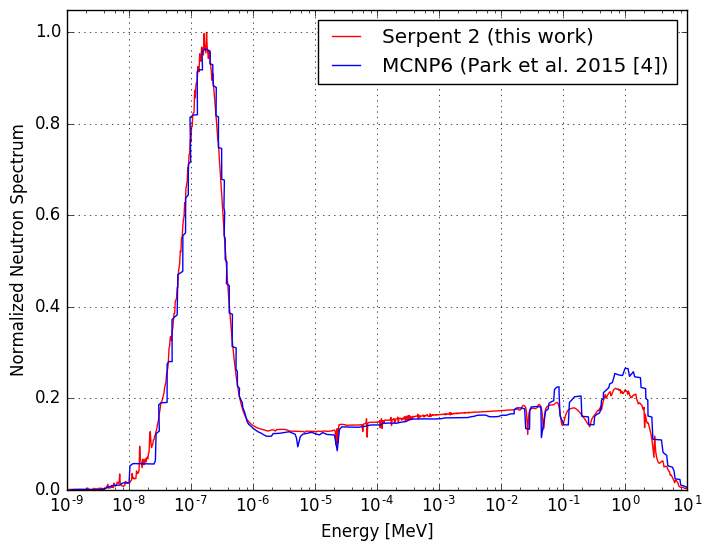
\includegraphics[width=\linewidth]{figure_3_1.png} 
  \caption{Neutron flux spectrum of MSBR for MCNP6 and Serpent 2 model.}
  \label{fig:spectrum}
\end{figure}
It is important to obtain the epithermal and thermal spectrum to produce $^{233}U$ from $^{232}Th$ because radiative capture cross section of thorium monotonically decreasing from $10^{-10} MeV$ to $10^{-5} MeV$. Hardening the spectrim tends to significantly increasing resonance absorbtion in thorium and decreasing the absorptions in fissile and construction materials thus large amount of fissile material will be needed to make the reactor critical.

\subsection{Effective multiplication factor}
Table~\ref{tab:keff} shows the effective multiplication factor for both MCNP6 and Serpent 2 whole core models. The coefficient obtained using Serpent 2 is about 4.37\% higher than MCNP6 one. The discrepancy was ocurred most likely because the model used in Park et al. didn't take into account $^{239}PuF_3$, contained in the fuel salt solution. Plutonium-239 has very high fission cross section in thermal energy range and produce more neutrons per fission than $^{233}U$, consequently, multiplication factor for this case is higher.
%%%%%%%%%%%%%%%%%%%%%%%%%%%%%%%%%%%%%%%%
\captionsetup[table]{
  labelsep = newline,
  name = TABLE, 
  justification=justified,
  singlelinecheck=false,%%%%%%% a single line is centered by default
  labelsep=colon,%%%%%%
  skip = \medskipamount}
\begin{table}[h!]
%\centering
\begin{tabular}{p{0.15\linewidth} p{0.3\linewidth} p{0.3\linewidth}} \toprule
      & Serpent2      & MCNP6 \cite{park_whole_2015}          
\\ \midrule
$K_{eff}$  & $1.05134\pm0.00116$ & $1.00736$
\\
\bottomrule
\end{tabular}
  \caption{Effective multiplication factor of whole core model.}
  \label{tab:keff}
\end{table}
%%%%%%%%%%%%%%%%%%%%%%%%%%%%%%%%%%%%%%%%%%%%%%%%%%%%%%%%%%%%%%%%%%%%%%%%%%%%%%%%
\subsection{Temperature effect of reactivity}
Table~\ref{tab:tcoef} represents the quantitive analysis of temperature effects on reactivity. Uncertainty for each temperature coefficient also was calculated and shown in Table~\ref{tab:tcoef}. The main physical principle underlying the reactor temperature feedback is expandsion of matter when it is heated. When the fuel salt temperature increases, the density of the salt decreases, but at the same time, the total volume of fuel salt in the core remains constant because it is defined by the space for fuel bounded by the graphite. When the reactor graphite temperature grows, the density of graphite declines which also frees up space for fuel salt. To determine temperature coefficients, three cases were considered:
\begin{enumerate}  
\item Temperature of fuel salt rising from 900K to 1200K.
\item Temperature of graphite rising from 900K to 1200K. 
\item Whole reactor temperature rising from 900K to 1200K.
\end{enumerate}

%%%%%%%%%%%%%%%%%%%%%%%%%%%%%%%%%%%%%%%%
\captionsetup[table]{
  labelsep = newline,
  name = TABLE, 
  justification=justified,
  singlelinecheck=false,%%%%%%% a single line is centered by default
  labelsep=colon,%%%%%%
  skip = \medskipamount}
\begin{table}[h!]
%\centering
\begin{tabular}{p{0.22\linewidth} p{0.22\linewidth} p{0.21\linewidth} p{0.15\linewidth}} \toprule
   Reactivity coefficient [pcm/K]  & Serpent2      & MCNP6 \cite{park_whole_2015}   & Reference \cite{robertson_conceptual_1971}      
\\ \midrule
Fuel salt        & $-3.93\pm0.005$ & $-3.20\pm0.05$ & $-3.22$ 
\\ \midrule
Moderator        & $+2.44\pm0.013$ & $-0.11\pm0.05$ & $+2.35$ 
\\ \midrule
Total            & $-1.74\pm0.030$ & $-3.21\pm0.04$ & $-0.87$ 
\\
\bottomrule
\end{tabular}
  \caption{Temperature coefficients of reactivity.}
  \label{tab:tcoef}
\end{table}
%%%%%%%%%%%%%%%%%%%%%%%%%%%%%%%%%%%%%%%%%%%%%%%%%%%%%%%%%%%%%%%%%%%%%%%%%%%%%%%%
On the one hand, changes in fuel temperature cause only density variation, geometry keeps the same because fuel is in the form of liquid. On the other hand, when moderator heats up both the density and the geometry changes due to thermal expansion of the graphite blocks and the reflector. New graphite density was calculated using linear temperature expansion coefficient of reactor graphite which is $1.3\times10^{-6}1/K$ \cite{robertson_conceptual_1971}. Based on this information new geometry input, which takes into account graphite expansion, was created.

The fuel temperature coefficient (FTC) is positive due to thermal Doppler broadening of the resonance capture cross sections in the thorium and is in a good agreement with early research \cite{robertson_conceptual_1971,park_whole_2015}. The moderator temperature coefficient is negative due to changing density, and would increases during reactor operation because of spectrum hardening along with fuel depletion \cite{park_whole_2015}. Finally, the total temperature coefficient of reactivity is relatively large and negative, despite graphite components, and affords excellent reactor stability and controllability.
%%%%%%%%%%%%%%%%%%%%%%%%%%%%%%%%%%%%%%%%%%%%%%%%%%%%%%%%%%%%%%%%%%%%%%%%%%%%%%%%
\section{Conclusions}
The MSBR full-core analysis was performed using the Serpent 2 Monte Carlo code. The complex geometry of the reactor is reconstructed in three-dimensional space without any major approximations. Accurate material data was employed to calculate reactor key design parameters. The effective multiplication factor for initial fuel composition is slightly higher than 1 (1.05) which allows reactor operation from startup to first online reprocessing cycle. The neutron flux energy spectrum was calculated for the whole core and represents the epithermal spectrum of the MSBR. The total temperature coefficient is negative, consequently, the MSBR has negative temperature feedback, but MTC is negative which has a negligible effect on safety because it is outweighed by the strong, negative FTC.

This high-fidelity full-core model will be employed for a number of future efforts. First, depletion simulation will be performed using built-in Serpent 2 depletion capabilities to find the equilibrium state of the MSBR, its optimal fuel salt composition, reprocessing characteristics (i.e. rates of removing fission products, the rate of adding thorium), and fuel utilization. Secondly, the model will be used to generate problem-oriented nuclear data libraries for multi-physics models of MSRs developed in the MOOSE-based coupled neutronics/thermal-hydraulics code Moltres \cite{lindsay_arfc/moltres:_2017}. Finally, transient accident simulations for safety investigation of the reactor core will be performed to study the dynamic behavior of Molten Salt Breeder Reactor. 


%%%%%%%%%%%%%%%%%%%%%%%%%%%%%%%%%%%%%%%%%%%%%%%%%%%%%%%%%%%%%%%%%%%%%%%%%%%%%%%%
\bibliographystyle{ans}
\bibliography{bibliography}
\end{document}

